
\documentclass[a4paper,10pt]{report}
\usepackage[utf8]{inputenc}
\usepackage[]{algorithm2e}
\usepackage[T1]{fontenc}
\usepackage{graphicx}

\begin{document}

\section*{Decomposição k-Core}


\subsection*{Definição}
 %TODO mudar anotações para equações
Sendo G = (V,E) um grafo com n = $|V|$ vértices e m = $|E|$ arestas, dG(u) o grau do vértice u, G(C) = $(C, E|C)$ um sub-grafo de G induzido pelo subconjunto de nós C onde $E|C = \{(u,v)\subset E : u,v \subset C\} $ temos as seguintes definições segundo Batagelj-Zaversnik:

\begin{enumerate}
	\item Um sub-grafo G(C) é uma k-core se e só se para todos os vértices pertencentes a C o seu grau é maior ou igual a k e G(C) e G(C) é um grafo maximal.
	\item Um nó de G diz-se ter \textit{coreness} se e só se este pertence à k-core mas não a (k+1)-core.
\end{enumerate}


Em outras palavras, é possível conseguir-se as k-Cores de G removendo recursivamente todos os vértices cujo grau sejam menor que k.

Assim, Batagelj-Zaversnik apresenta este algoritmo para determinar a hierarquia das \textit{core} de um grafo:

%INPUT: graph G = (V,L) represented by lists of neighbors Neighbors(v) for
%each vertex v
%OUTPUT: table core with core number core[v] for each vertex v
%1.1 compute the degrees of vertices;
%1.2 order the set of vertices V in increasing order of their degrees;
%2 for each v ∈ V in the order do begin
%2.1 core[v] := degree[v];
%2.2 for each u ∈ Neighbors(v) do
%2.2.1 if degree[u] > degree[v] then begin
%2.2.1.1 degree[u] := degree[u] − 1;
%2.2.1.2 reorder V accordingly
%end
%end;

\begin{algorithm}[H]
 \KwData{graph G = (V,L) represented by lists of neighbors Neighbors(v) for each vertex v}
 \KwResult{table core with core number core[v] for each vertex v }
 compute the degrees of vertices\;
 \ForEach{$v$ in $V$ in the order}{
  core[v] := degree[v]\;
  \ForEach{$u$ in $Neighbors(v)$ }{
		\If{ degree[u] > degree[v] }{
			degree[u] := degree[u]-1\;
			reorder V accordingly\;
		}
  }
 }
\end{algorithm}

Onde o ciclo sobre os vizinhos de v simula a remoção deste vértice e o efeito disto sobre os seus vizinhos - o grau destes é reduzido por um visto que deixa de existir a aresta proveniente de v.
Após a remoção a lista de vizinhos, u é removido de V e V é reordenada de modo a garantir a ordem crescente onde o grau de uma vértice v é o final quando esta é removida do grafo 
%Imagem aqui


\subsection*{Decomposição k-Core distribuída}
O algoritmo de decomposição central referido em cima requer que todo o grafo esteja em memória, o que não pode ser possível para grafos de grande escala. Devido a isto, em Distributed k-Core Decomposition, é apresentado um outro algoritmo para a decomposição k-Core distribuída.


\begin{figure}[ht!]
%\centering
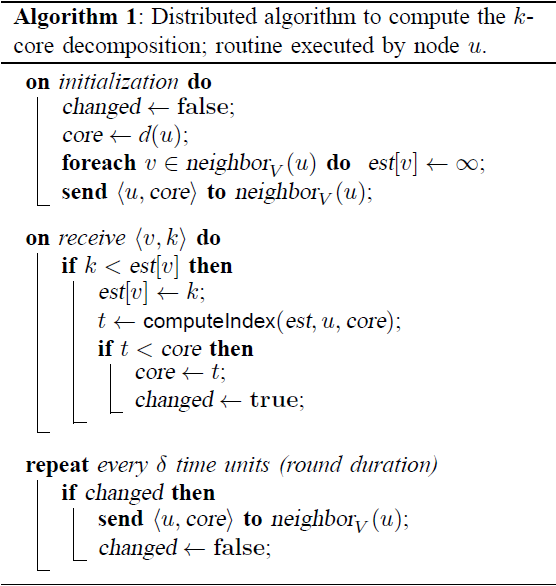
\includegraphics[width=90mm]{Algorithm1}
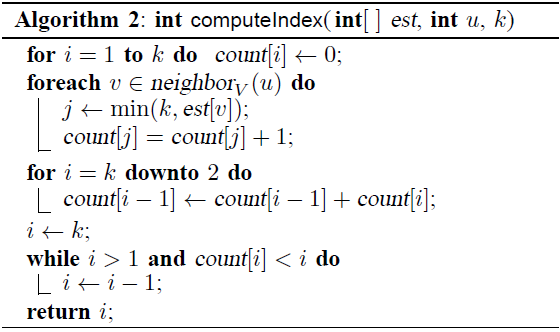
\includegraphics[width=90mm]{Algorithm2}
\label{overflow}
\end{figure}
%Distributed k-Core Decomposition

%http://arxiv.org/pdf/1103.5320v2.pdf

%http://arxiv.org/pdf/cs/0310049v1.pdf
\end{document}